% !TeX spellcheck = en_GB
%
\documentclass[presentation]{beamer}
\mode<presentation>{\usetheme{AMSCesenaPurpleAndGold}}
\setbeamertemplate{bibliography item}{\insertbiblabel}
\setbeamersize{description width=0.57cm}
%%%%%%%%%%%%%%%%%%%%%%%%%%%%%%%%%%%%%%%%%%%%%%%%%%%%%%%%%%%%%%%%%%%%%%%%%%%%%%%%
\usepackage{2p-kt-talk}
%%%%%%%%%%%%%%%%%%%%%%%%%%%%%%%%%%%%%%%%%%%%%%%%%%%%%%%%%%%%%%%%%%%%%%%%%%%%%%%%
\title[\twopkt]{
    \twopkt{}: A Kotlin Multi-Platform ecosystem for Symbolic AI
}
%
% \subtitle{Extended Abstract}
%
% same authors order of the presented paper
\author[Ciatto, Rizzato]{
    \emph{Giovanni Ciatto}$^{1}$ % empth the presenting author
    \and
    Lorenzo Rizzato$^{2}$
}
%
\institute[UniBo]{
    $^{1}$ Dipartimento di Informatica -- Scienza e Ingegneria (DISI)
    \\
    \textsc{Alma Mater Studiorum} -- Università di Bologna
    \\
    \texttt{
        giovanni.ciatto@unibo.it % emph the presenting author's email
    }
    \and
    $^{2}$\texttt{lorenzo.rizzato@studio.unibo.it}
}
%
\date[A.Y. 20-21]{
    Autonomous Systems Course, A.Y. 2020-2021
}
%%%%%%%%%%%%%%%%%%%%%%%%%%%%%%%%%%%%%%%%%%%%%%%%%%%%%%%%%%%%%%%%%%%%%%%%%%%%%%%%
\AtBeginSection[]{
    \begin{frame}<beamer>[shrink,noframenumbering]\frametitle{Next in Line\ldots}
        \mbox{~}
        \tableofcontents[sectionstyle=show/shaded,subsectionstyle=hide,subsubsectionstyle=hide]
        \mbox{~}
    \end{frame}
}
\AtBeginSubsection[]{
    \begin{frame}<beamer>[shrink,noframenumbering]\frametitle{Focus on\ldots}
        \mbox{~}
        \tableofcontents[sectionstyle=show/shaded,subsectionstyle=show/shaded,subsubsectionstyle=hide]%[currentsection,currentsubsection,sectionstyle=shaded,subsectionstyle=shaded,subsubsectionstyle=hide]
        \mbox{~}
    \end{frame}
}
%%%%%%%%%%%%%%%%%%%%%%%%%%%%%%%%%%%%%%%%%%%%%%%%%%%%%%%%%%%%%%%%%%%%%%%%%%%%%%%%
\begin{document}
%%%%%%%%%%%%%%%%%%%%%%%%%%%%%%%%%%%%%%%%%%%%%%%%%%%%%%%%%%%%%%%%%%%%%%%%%%%%%%%%

%\\\\\\\\\\\\\\\\\\\\\
\frame{\titlepage}
%\\\\\\\\\\\\\\\\\\\\\

\begin{frame}<beamer>[shrink,noframenumbering]\frametitle{Outline}
    \mbox{~}
    \tableofcontents
    \mbox{~}
\end{frame}

\section{Historical Perspective}

\subsection{Prolog History}

\begin{frame}{Implementations of Prolog -- Chronological Perspective}
    % !TEX root = 2p-kt-talk.tex
\begin{figure}[h]\centering
    \tiny
    \catcode`\@=11
    \def\chron@selectmonth#1{\ifcase#1\or January\or February\or
    March\or April\or May\or June\or
    July\or August\or September\or
    October\or November\or December\fi}
    \startchronology[startyear=1972,startdate=false,stopdate=false,stopyear=1995]
    \chronoevent[markdepth=-20pt]{1972}{1st Prolog}
    \chronoevent{1973}{Final Marseille's Prolog}
    \chronoevent[markdepth=-20pt]{1977}{Prolog II}
    \chronoevent[markdepth=40pt]{1977}{DEC-10 Prolog}
    \chronoevent[markdepth=-20pt]{1982}{C-Prolog}
    \chronoevent[markdepth=10pt]{1983}{\textbf{\emph{(The WAM)}}}
    \chronoevent[markdepth=-50pt]{1984}{Quintus}
    \chronoevent[markdepth=-20pt]{1986}{SICStus~ ~}
    \chronoevent[markdepth=40pt]{1986}{\&-Prolog/Ciao}
    \chronoevent[markdepth=-20pt]{1988}{~CLP(R)} % Could be in 87 also, but does not fit
    \chronoevent[markdepth=-50pt]{1987}{SWI-Prolog}
    \chronoevent[markdepth=10pt]{1988}{SB-Prolog}
    \chronoevent[markdepth=-50pt]{1990}{\eclipse{}}
    \chronoevent[markdepth=40pt]{1991}{BinProlog}
    \chronoevent[markdepth=-20pt]{1993}{XSB}
    \chronoevent[markdepth=5pt]{1993}{wamcc}
    \chronoevent[markdepth=40pt]{1994}{B-Prolog}
    \chronoevent[markdepth=15pt]{1995}{GNU Prolog}
    \chronoevent[markdepth=-50pt]{1995}{\textbf{\emph{(ISO Prolog)}}}
    % SICStus, YAP somewhat unclear
    % Cannot fit MU-Prolog...
    \stopchronology
    % \caption{Timeline of Early Prolog-Related Systems (up to the ISO Standard)}%
    \label{fig:timeline}
\end{figure}
\end{frame}

\begin{frame}{Implementations of Prolog -- Familiy Tree}
    % !TEX root = 2p-kt-talk.tex
\begin{figure}
\tikzstyle{inactive}=[rectangle, draw=black, rounded corners, fill=gray!50, drop shadow,
        text centered, anchor=north, text=black]
\tikzstyle{active}=[rectangle, draw=black, rounded corners, fill=white, drop shadow,
        text centered, anchor=north, text=black]
\tikzstyle{myarrow}=[->, >=open triangle 90, thick]
\tikzstyle{line}=[-, thick]

\pgfdeclarelayer{background}
\pgfdeclarelayer{foreground}
\pgfsetlayers{background,main,foreground}
\usetikzlibrary{positioning}
\begin{adjustbox}{width=.8\textwidth}    
    \begin{tikzpicture}[node distance=.6cm]
    % \node (Prolog0) [inactive, rectangle split, rectangle split parts=2]
    %     {
    %         \textbf{Prolog 0}
    %         \nodepart{second}{\scriptsize first Prolog System}
    %     };
    \node (Prolog1) [inactive, rectangle split, rectangle split parts=2]
        {
            \textbf{Prolog 0 \& I}
            \nodepart{second}{\scriptsize negation as failure}
        };
    % \draw[-Stealth] (Prolog0.south) -- (Prolog1.north) ;

    \node (Prolog2) [inactive, rectangle split, rectangle split parts=2, below=of Prolog1]
        {
            \textbf{Prolog II}
            \nodepart{second}{\scriptsize cyclic structures}
        };
    \draw[-Stealth] (Prolog1.south) -- (Prolog2.north) ;

    \node (Prolog3) [inactive, rectangle split, rectangle split parts=2, below=of Prolog2]
        {
            \textbf{Prolog III}
            \nodepart{second}{\scriptsize constraints}
        };
    \draw[-Stealth] (Prolog2.south) -- (Prolog3.north) ;

    \node (Prolog4) [inactive,
      % rectangle split, rectangle split  parts=2,
    below=of Prolog3]
        {
            \textbf{Prolog IV}
            % \nodepart{second}{\scriptsize constraints}
        };
    \draw[-Stealth] (Prolog3.south) -- (Prolog4.north) ;

    \node (DEC10) [inactive, rectangle split, rectangle split parts=2, right=of Prolog1, yshift=-3mm]
        {
            \textbf{DEC-10 Prolog}
            \nodepart{second}{\scriptsize compiled, de facto standard}
        };
    \draw[-Stealth] (Prolog1.east) -- (DEC10.west);

    \node (CProlog) [inactive, rectangle split, rectangle split parts=2, right=of DEC10, yshift=-2mm]
        {
            \textbf{C-Prolog}
            \nodepart{second}{\scriptsize interpreted, portable}
        };
    \draw[-Stealth] (DEC10.east) -- (CProlog.west);

    \node (WAM) [inactive, rectangle split, rectangle split parts=2, below=of DEC10, yshift=1mm]
        {
            \textbf{The WAM} % Warren Abstract Machine (WAM)
            \nodepart{second}{\scriptsize compiled, portable}
        };
    \draw[-Stealth] (DEC10.south) -- (WAM.north);
    \node (Quintus) [inactive, rectangle split, rectangle split parts=2, below=of WAM, yshift=2mm]
        {
            \textbf{Quintus}
            \nodepart{second}{\scriptsize commercial, de-facto standard}
        };
    \draw[-Stealth] (WAM.south) -- (Quintus.north);

    \node (SICStus) [active, rectangle split, rectangle split parts=2, below=of Quintus, yshift=3mm]
        {
            \textbf{SICStus}
            \nodepart{second}{\scriptsize commercial support, JIT}
        };
    \draw[-Stealth] (Quintus.south) -- (SICStus.north);

    \node (BIM) [inactive, rectangle split, rectangle split parts=2, right=of Quintus, xshift=6mm, yshift=-4mm]
        {
            \textbf{BIM} % -Prolog
            \nodepart{second}{\scriptsize commercial, native}
        };
    \draw[-Stealth] (WAM.east) -| (BIM.north);

    \node (Ciao) [active, rectangle split, rectangle split parts=2, below=of SICStus, yshift=3mm]
        {
            \textbf{\&-Prolog/Ciao}
            \nodepart{second}{\scriptsize parallel, assertions}
        };
    \draw[-Stealth] (SICStus.south) -- (Ciao.north);

    \node (SWI) [active, rectangle split, rectangle split parts=2, right=of Ciao]
        {
            \textbf{\ SWI\ } % SWI-Prolog
            \nodepart{second}{\scriptsize libraries}
        };
    \draw[-Stealth] (Quintus.south east) -- (SWI.north);

    \node (YAP) [active, rectangle split, rectangle split parts=2, right=of SWI]
        {
            \textbf{YAP} % -Prolog
            \nodepart{second}{\scriptsize indexing}
        };
    \draw[-Stealth] (Quintus.east) -- (YAP.north west);

    \node (SB) [inactive,
    % rectangle split, rectangle split parts=2,
    right=of YAP]
        {
            \textbf{SB-Prolog}
            \nodepart{second}
        };
    \draw[-Stealth] (WAM.east) -| (SB.north);

    \node (XSB) [active, rectangle split, rectangle split parts=2, below=of SB]
        {
            \textbf{XSB}
            \nodepart{second}{\scriptsize tabling}
        };
    \draw[-Stealth] (SB.south) -- (XSB.north);

    \node (GNU) [active, rectangle split, rectangle split parts=2, right=of XSB]
        {
            \textbf{GNU} % -Prolog
            \nodepart{second}{\scriptsize fd/indexicals}
        };
    \draw[-Stealth] (WAM.east) -| (GNU.north);

    \node (OtherW) [active, right=of GNU, xshift=-2mm]
        {
            \textbf{\ \ \ldots\ \ }
        };

    \node (BProlog) [active, rectangle split, rectangle split parts=2, left=of XSB]
        {
            \textbf{B-Prolog}
            \nodepart{second}{\tiny TOAM}
        };
    \draw[-Stealth] (SB.south west) -- (BProlog.north east);

    \node (Bin) [active, rectangle split, rectangle split parts=2, left=of BProlog, xshift=3mm]
        {
            \textbf{BinProlog}
            \nodepart{second}{\scriptsize binarization}
        };

    \node (tuProlog) [active, rectangle split, rectangle split parts=2, left=of Bin, xshift=3mm]
        {
            \textbf{tuProlog}
            \nodepart{second}{\scriptsize jvm, interop.} % interoperability
        };

    \node (OtherNW) [active, below=of BProlog, xshift=3mm, yshift=4mm]
        {
            \textbf{\ \ \ldots\ \ } 
        };

    \node (Marseille1) [below= 2mm of Prolog4]
        {
            \textbf{Marseille}
        };
    \node (Marseille2) [below= -1mm of Marseille1]
        {
            \textbf{Prolog-line}
        };

    \node (WAM-comment2) [right=of Quintus, xshift=-2mm, yshift=4mm]
        {
            \textbf{Prologs}
        };
    \node (WAM-comment1) [above=0mm of WAM-comment2]
        {
            \textbf{WAM-based}
        };
    % \node (WAM-comment) [below= 1mm of GNU, align=right,xshift=-6mm]
    %     {
    %         \textbf{WAM-based Prologs}
    %     };

    \node (NWAM-comment) [below=1mm of tuProlog,align=right,xshift=5mm]
        {
            \textbf{WAM alternatives}
        };

        \begin{pgfonlayer}{background}
        \path (Prolog1.west |- Prolog1.north)+(-0.2,0.2) node (a) {};
        \path (Marseille2.east |- Marseille2.south)+(+0.3,0) node (c) {};
        \path[fill=gray!5,rounded corners, draw=black!50, dashed]
              (a) rectangle (c);

        \path (Quintus.west |- WAM.north)+(-0.2,0.2) node (wam-a) {};
        \path (OtherW.east |- GNU.south)+(+0.2,-0.2) node (wam-c) {};
        \path[fill=gray!5,rounded corners, draw=black!50, dashed]
              (wam-a) rectangle (wam-c);

        \path (tuProlog.west |- tuProlog.north)+(-0.2,0.2) node (nwam-a) {};
        \path (BProlog.east |- NWAM-comment.south)+(+0.3,-0.1) node (nwam-c) {};
        \path[fill=gray!5,rounded corners, draw=black!50, dashed]
              (nwam-a) rectangle (nwam-c);
        \end{pgfonlayer}
    \end{tikzpicture}
\end{adjustbox}
\caption{Prolog implementations in perspective. Notice the pivotal role of the WAM \cite{Warren1983}}
\end{figure}

\end{frame}

\begin{frame}[allowframebreaks]{Implementations of Prolog -- Features}
    % !TEX root = 2p-kt-talk.tex
\centering

\begin{adjustbox}{width=.8\textwidth} 
    \begin{tabular}{|l|ccccccc|}
        \hline
        System            & Open Source  & Modules  & Tabling  & Parallelism  & CLP            & CHR      & Global Variables  \hfill \\
        \hline\hline
        B-Prolog          & \xmark       & \xmark   & \cmark   & \xmark       & FD, B, Set     & (\cmark) & \cmark \\
        Ciao              & \cmark       & \cmark   & \cmark   & \cmark       & Q, R, FD       & \cmark   & \cmark \\
        ECLiPSe           & \cmark       & \cmark   & \xmark   & \cmark       & FD, Q, R, Set  & \cmark   & \cmark \\
        GNU Prolog        & \cmark       & \xmark   & \xmark   & \xmark       & FD, B          & \xmark   & \cmark \\
        Jekejeke          & \xmark       & \cmark   & \xmark   & \cmark       & FD, B          & \cmark   & \xmark \\
        JIProlog          & \cmark       & \cmark   & \xmark   & \xmark       & \xmark         & \xmark   & \xmark \\
        SWI               & \cmark       & \cmark   & \cmark   & \cmark       & FD, B, Q, R    & \cmark   & \cmark \\
        SICStus           & \xmark       & \cmark   & \xmark   & \xmark       & FD, B, Q, R    & \cmark   & \xmark \\
        tauProlog         & \cmark       & \cmark   & \xmark   & \xmark       & \xmark         & \xmark   & \xmark \\
        tuProlog          & \cmark       & \xmark   & \xmark   & \cmark       & \xmark         & \xmark   & \xmark \\
        XSB               & \cmark       & \cmark   & \cmark   & \cmark       & R              & \cmark   & \xmark \\
        YAP               & \cmark       & \cmark   & \cmark   & \xmark       & \cmark         & \cmark   & \cmark \\
        \hline
    \end{tabular}
\end{adjustbox}

\framebreak

\begin{adjustbox}{width=.8\textwidth} 
    \begin{tabular}{|l|cccccc|}
        \hline
        System            &  Indexing       & Type / Mode & Co-Routines  & Testing      & Debugger          & Mutable Terms \hfill\\
        \hline\hline
        B-Prolog          &  N-FA           & \xmark      & (\cmark)     & \xmark       & trace             & \xmark \\
        Ciao              &  FA, MA         & \cmark      & \cmark       & \cmark       & trace / source    & \cmark \\
        ECLiPSe           &  most suitable  & \xmark      & \cmark       & \cmark       & trace             & \xmark \\
        GNU Prolog        &  FA             & \xmark      & \xmark       & \xmark       & trace             & \cmark \\
        Jekejeke          &  FA, N-FA, MA   & \xmark      & \cmark       & \xmark       & spy               & \xmark \\
        JIProlog          &  undocumented   & \xmark      & \xmark       & \xmark       & trace             & \xmark \\
        SWI               &  JIT, MA, deep  & \xmark      & \cmark       & \cmark       & trace / graphical & \cmark \\
        SICStus           &  FA             & \xmark      & \cmark       & \cmark       & trace / source    & \cmark \\
        tauProlog         &  undocumented   & \xmark      & \xmark       & \xmark       & \xmark            & \xmark \\
        tuProlog          &  FA             & \xmark      & \xmark       & \xmark       & spy               & \xmark \\
        XSB               &  all, trie      & \xmark      & \cmark       & \xmark       & trace             & \xmark \\
        YAP               &  FA,MA,jit      & \xmark      & \xmark       & \xmark       & trace             & \xmark \\
        \hline
    \end{tabular}
\end{adjustbox}

\framebreak

\begin{adjustbox}{width=.5\textwidth} 
    \begin{tabular}{|l|cc|}
        \hline
        System            & FLI                  & Non-Standard Data Types     \\ 
        \hline\hline
        B-Prolog          & C, Java              & arrays, sets, hashtables               \\
        Ciao              & C, Java, Python, JS  & \xmark\\
        ECLiPSe           & C, Java, Python, PHP & arrays, strings,         \\
        Jekejeke          & Java                 & arrays          \\
        JIProlog          & Java                 & \xmark \\
        GNU Prolog        & C, Java, PHP         & arrays          \\
        tauProlog         & JavaScript           & \xmark          \\
        tuProlog          & Java, .NET, Android, iOS           & arrays          \\
        SWI               & C, C++, Java         & dicts, strings \\
        SICStus           & C, Java, .NET, Tcl/Tk & \xmark              \\
        XSB               & C, Java, PERL        & \xmark                \\
        YAP               & C, Python, R         & \xmark                \\
        \hline
    \end{tabular}
\end{adjustbox}


\end{frame}

\subsection{\tuprolog{} History}

\begin{frame}[allowframebreaks]{\tuprolog{} History}
\begin{block}{Foundational features and ideas}
	\begin{itemize}
		\item light-weight Prolog system for \alert{distributed} applications and infrastructures \ccite{tuprolog-padl01}
		\item intentionally designed around a \alert{minimal core}
		\item to be either statically or dynamically \emph{configured} by loading/unloading \alert{libraries} of predicates
		\item \tuprolog{} natively supports \alert{multi-paradigm programming} \ccite{tuprolog-scp57}, providing a clean, seamless integration model between Prolog and mainstream object-oriented languages
	\end{itemize}
\end{block}

\framebreak

\begin{itemize}
	\item first release lightweight Prolog solver written in Java \ccite{tuprolog-padl01}
	\begin{itemize}
		\item state of the art advancements: OOP-interoperable, and SM-based \ccite{weblp-ia5}
	\end{itemize}
	\item extended along many research directions
	\begin{description}
		\item[LPaaS] micro-intelligence vision (lightweight logic solvers running on most devices) for IoT and Cloud/Edge computing \ccite{lpaas-tplp18}
		\item[TuSoW] bringing tuple-based coordination at the edge \ccite{tusow-icccn2019}
	\end{description}
	\item foundation of many research projects
	\begin{description}
		\item[TuCSoN / ReSpecT] coordination model for Internet applications based on network-aware and mobile agents \ccite{tucson-jaamas2} by means of reactions to communication events \ccite{respect-scp41}
		\item[MoK] self-organising knowledge-oriented model based on biochemical tuple space \ccite{mok-idc2012}
		\item[Arg2P] defeasible reasoning and argumentation tool \ccite{arg2p-cilc2020}
	\end{description}
\end{itemize}

\framebreak

\begin{itemize}
	\item[$\rightarrow$] legacy code: making it Prolog-constrained and hard to maintain
	\item[$\rightarrow$] complete re-design and re-write as Kotlin MPP
	\begin{itemize}
		\item[$\Rightarrow$]  widening the scope to whole LP rather than Prolog alone
	\end{itemize}
\end{itemize}

\end{frame}

\section{Motivation}

\begin{frame}{Why \twopkt{}}
    \begin{itemize}
        \item Building an open an extensible ecosystem\ldots
        \vfill
        \item \ldots supporting \alert{multiple logics} (e.g. FOL, DL, TL, BDI, etc)
        %
        \begin{itemize}
            \item via as many \alert{inference rules} as possible (e.g. deduction, abduction, induction)
            %
            \begin{itemize}
                \item implemented, in turn, via multiple \alert{resolution strategies} (e.g. SLDNF, IFF, Probabilistic, etc.)
            \end{itemize}
        \end{itemize}
        \vfill
        \item Making each aspect of LP individually usable \emph{per se}
        \vfill
        \item Reaching widest possible platform support
        \vfill
        \item Blending LP with OOP and FP
        \vfill
        \item Bridging symbolic and sub-symbolic AI
    \end{itemize}
\end{frame}

\begin{frame}{Which features of LP}
    \begin{enumerate}
        \item Knowledge representation: \alert{terms}, and \alert{clauses}
        \vfill
        \item \alert{Unification}, based on \cite{MartelliMontanari1982} but possibly customisable
        \vfill
        \item Clauses \alert{indexing} and in-memory \alert{storage} facilities for \alert{knowledge bases}
        \vfill
        \item Prolog-like syntax \alert{parsing} \& \alert{formatting}
        \vfill
        \item \alert{Serialization} / \alert{deserialization} of terms, clauses, and knowledge bases
        \vfill
        \item Generic \alert{resolution} API, possibly customisable via \alert{pluggable features}
        \vfill
        \item \alert{SLD NF} (Prolog-like) resolution streategy \cite{Robinson65SLD,Clark77}
        \vfill
        \item Support for other resolution strategies
        \vfill
        \item Common \alert{UI} facilities
        \vfill
        \item[\vdots]
    \end{enumerate}
\end{frame}

\begin{frame}{Why Kotlin}
    \begin{itemize}
        \item Multi-platform support:
        %
        \begin{itemize}
            \item JVM (Win + Linux + Mac)
            \item JS (Web, both browser and server side)
            \item Android
            \item Native?
            \item iOS?
        \end{itemize}

        \vfill

        \item Good platform-specific interoperability
        %
        \begin{itemize}
            \item Kotlin libraries can easily be exploited in bare Java projects
            \item Kotlin libraries can be exploited in bare JavaScript projects
        \end{itemize}

        \vfill

        \item Clean and practical framework and tool-kit available
    \end{itemize}
\end{frame}

\section{Overview of the Project}

\begin{frame}[allowframebreaks]{Project Map}
    \begin{itemize}
        \item \twopkt{} is an ecosystem of \alert{modules}
        %
        \begin{itemize}
            \item denoted by Gradle's notation: \module{moduleName}
        \end{itemize}

        \medskip

        \item Modules are \alert{loosely-coupled}, yet incrementally inter-dependent
        %
        \begin{itemize}
            \item[$\rightarrow$] \alert{onion-like} architectural design
        \end{itemize}

        \medskip

        \item Modules are compilation and \alert{deployment units}
        %
        \begin{itemize}
            \item 1 module $\leftrightarrow$ 1 jar, on the JVM
        \end{itemize}

        \medskip

        \item Using a module as a dependecy $\implies$ importing \alert{all} its dependencies
    \end{itemize}

    \framebreak

    \begin{center}
        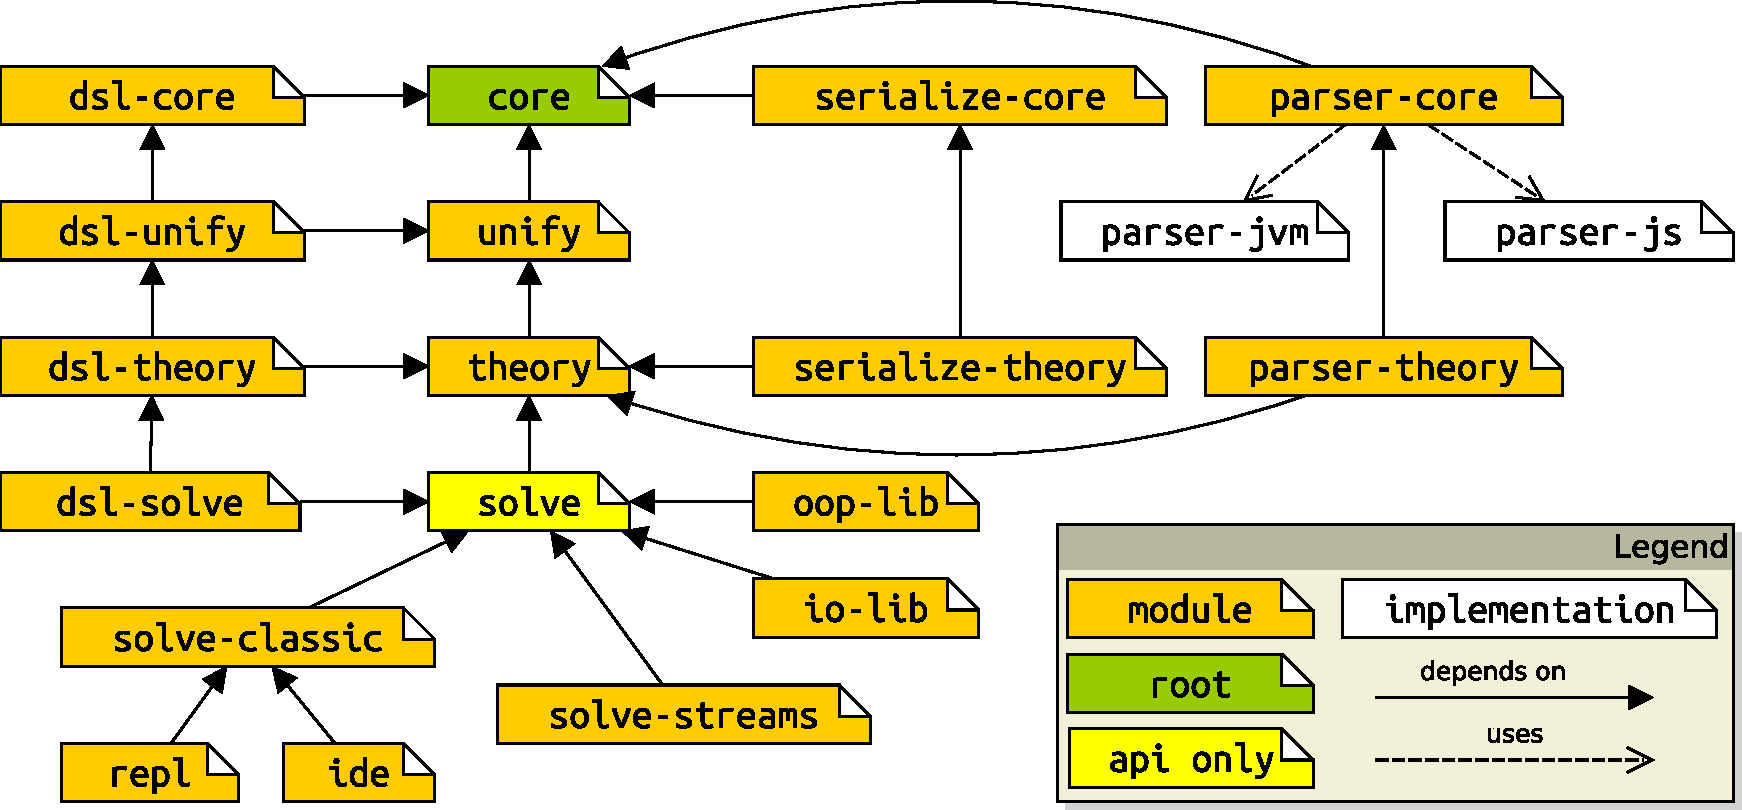
\includegraphics[width=\linewidth]{img/project-map.pdf}
    \end{center}

    \framebreak

    \begin{description}
        \item[\module{core}] provides \alert{knowledge representations} facilities \& common features
        %
        \begin{itemize}\small
            \item[eg] terms, clauses, substitutions, operators, term formatting, basic exceptions, etc.
        \end{itemize}

        \medskip

        \item[\module{unify}] provides support for \alert{logic unification}
        %
        \begin{itemize}\small
            \item[eg] customisable notion of unificator based on \cite{MartelliMontanari1982}
        \end{itemize}

        \medskip

        \item[\module{theory}] provides support in-memory \alert{storage \& indexing} of clauses
        %
        \begin{itemize}\small
            \item[eg] mutable/immutable and ordered/unordered \alert{collections of clauses} + \alert{logic theories}
        \end{itemize}

        \medskip

        \item[\module{solve}] provides generic support for \alert{resolution-related} stuff
        %
        \begin{itemize}\small
            \item[!] agnostic w.r.t. inference procedures \& resolution strategy
            \item[eg] solvers, solutions, libraries, errors, flags, channels, etc.
        \end{itemize}

        \framebreak

        \item[\module{solve-*}] provide specific implementation for inference procedures \& \alert{resolution} strategy
        %
        \begin{description}\small
            \item[\module{solve-classic}] SLD NF (Prolog-like) resolution \cite{Robinson65SLD,Clark77} based on Piancastelli's state machine \cite{tuprolog-sac08} (\alert{Prolog ISO \cite{prologISO-pt1} Compliant})
            \item[\module{solve-streams}] SLD NF (Prolog-like) resolution \cite{Robinson65SLD,Clark77} based on Enrico Siboni's master thesis and on \cite{Carlsson84}
        \end{description}

        \medskip

        \item[\module{parser-*}] supports \alert{parsing} of terms and clauses in Prolog syntax
        %
        \begin{description}\small
            \item[\module{parser-core}] supports parsing terms
            \item[\module{parser-theory}] supports parsing knowledge bases and streams of clauses
            \item[\module{parser-jvm/js}] platform-specific implementations, based on ANTLR \cite{Parr2013} \hint{(not to be used directly!)}
        \end{description}

        \framebreak

        \item[\module{serialization-*}] support \alert{(de)serialization} of terms, clauses, knowledge bases in \alert{YAML/JSON}
        %
        \begin{description}\small
            \item[\module{serialization-core}] (de)serialization of terms and clauses
            \item[\module{serialization-theory}] (de)serialization of knowledge bases and theories
        \end{description}

        \medskip

        \item[\module{dsl-*}] incrementally support the Kotlin-based DSL for LP described in~\cite{kotlinDSl4PrologWoa2020}, aimed at blending LP, FP, and OOP
        %
        \begin{description}\small
            \item[\module{dsl-core}] basic DSL for building terms/clauses in Kotlin
            \item[\module{dsl-unify}] extension of the DSL incuding \module{unify} facilities
            \item[\module{dsl-theory}] extension of the DSL incuding \module{theory} facilities
            \item[\module{dsl-solve}] extension of the DSL incuding \module{solve} facilities
        \end{description}

        \framebreak

        \item[\module{repl}] command-line interface for Prolog

        \medskip

        \item[\module{ide}] JavaFX-based GUI for Prolog (customisable)

        \medskip

        \item[\module{io-lib}] Prolog ISO compliant Prolog library for I/O

        \medskip

        \item[\module{oop-lib}] Prolog library for OOP interoperability
        %
        \begin{itemize}\small
            \item essentially, lets Kotlin's and Java's OOP facilities be exploited from LP
            \item only JVM is currently supported, due to limitations in Kotlin's reflection API
        \end{itemize}

    \end{description}
\end{frame}

\section{Knowledge Representation: the \module{core} Module}

\begin{frame}[allowframebreaks]{Main Abstractions from the \module{core} Module}
    \begin{block}{Terms and Clauses}\center\itshape\small
        Immutable data structures for terms and clauses in-memory representation \& manipulation
    \end{block}

    \begin{block}{Substitutions}\center\itshape\small
        Immutable data structures representing variables assignments, applicable to terms/clauses
    \end{block}

    \begin{block}{Operators and Operators Sets}\center\itshape\small
        Immutable data strucuters for representing logic operators and their esembles
    \end{block}

    \framebreak

    \begin{block}{Formatters}\center\itshape\small
        Functional objects aimed at converting terms/clauses into strings of customisable format
    \end{block}

    \begin{block}{Visitors}\center\itshape\small
        Functional objects aimed at easing type-dependent algorithms writing
    \end{block}

    \begin{block}{Exceptions}\center\itshape\small
        Base exception types extensively exploited in all whole \twopkt{} project
    \end{block}
\end{frame}

\subsection{The \kt{Term} Hierarchy}

\subsubsection{Main Sorts of \kt{Term}s and \kt{Clause}s}

\begin{frame}[allowframebreaks]{Term Hierarchy}
    \begin{center}
        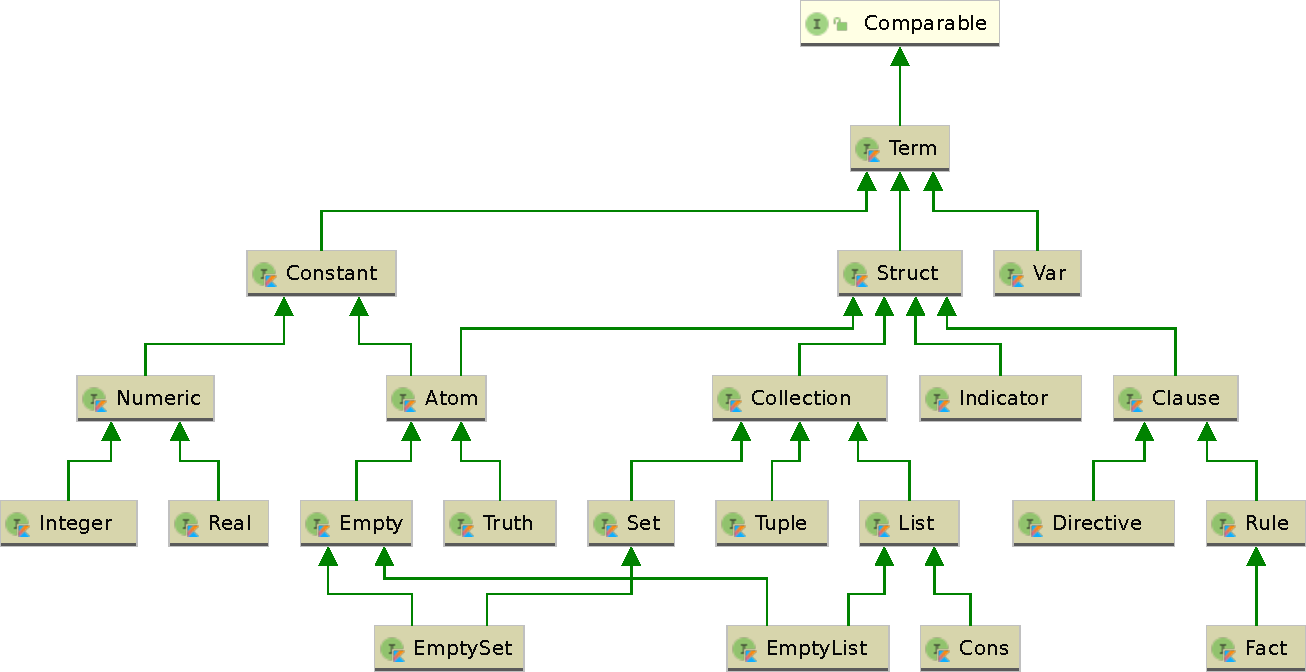
\includegraphics[width=\linewidth]{img/TermHierachy.pdf}
    \end{center}

    \begin{block}{Common Conventions}
        \begin{itemize}
            \item Only intefaces are publicly available, no classes
            \item Immutable design: all terms are immutable data structures
            \item The hierarchy is a DAG, not a tree
            \item Terms are totally ordered, as the are \kt{Comparable} among each others
            \item We call ``term'' any object which (indirectly) implements \kt{Term}
            %
            \begin{itemize}
                \item[!] there including clauses, i.e. instances of \kt{Clause}
            \end{itemize}
        \end{itemize}
    \end{block}
\end{frame}

\begin{frame}[allowframebreaks]{The \kt{Term} type}
    \begin{block}{The \kt{Term} type}\centering
        Base type for all terms
    \end{block}
    %
    \begin{description}
        \item[\kt{is\meta{SubType}: Boolean}] checks whether the current term is an instance of \kt{\meta{SubType}} or not
        \item[\kt{as\meta{SubType}(): \meta{SubType}}] casts the current term to \kt{\meta{SubType}} or returns null if not possible
        \item[\kt{castTo\meta{SubType}(): \meta{SubType}}] casts the current term to \kt{\meta{SubType}} or throws an exception if not possible
        \item[\kt{freshCopy(): Term}] returns a deep copy of the current term where all \kt{Var}iables have been refreshed
        \item[\kt{apply(Substitution): Term}] applies the provided \kt{Substitution} to the current \kt{Term} or throws a \kt{SubstitutionApplicationException} in case a failed \kt{Substitution} has been provided
        \item[\kt{equals(Term, Boolean): Boolean}] checks whether the provided \kt{Term} is deeply equal to the current one, letting the caller choose whether to compare variables by simple or by complete name
        \item[\kt{equals(Any?): Boolean}] checks whether the provides object is a \kt{Term} is deeply equal to the current one, comparing variables by complete names
        \item[\kt{structurallyEquals(Term): Boolean}] checks whether the provided \kt{Term} is deeply equal to the current one, in such a way that all variables are considered equal
        \item[\kt{accept<T>(TermVisitor<T>): T}] returns the object produced by letting the provided \kt{TermVisitor} visit the current \kt{Term}
        \item[\kt{compareTo(Term): Int}] compares the current \kt{Term} with the provided one, according to the total ordering on \kt{Term}s
        \item[\kt{toString(): String}] returns a representation of the current \kt{Term} for debugging purposes
    \end{description}
\end{frame}

\begin{frame}[allowframebreaks]{Main Sorts of \kt{Term}s}
    \begin{block}{The \kt{Constant} type is a sub-type of \kt{Term}}\centering
        Base type for all constant terms (namely, strings and numbers)
    \end{block}
    %
    \begin{description}
        \item[\kt{value: Any}] returns the value of this \kt{Constant}
    \end{description}

    \framebreak

    \begin{block}{The \kt{Numeric} type is a sub-type of \kt{Constant}}\centering
        Base type for all numeric terms (namely, reals and integers)
    \end{block}
    %
    \begin{description}
        \item[\kt{intValue: BigInteger}] returns the integer value of the current number
        %
        \begin{itemize}
            \item \kt{BigInteger}s can then be converted into \kt{Int}, \kt{Short}, etc.
            \item unlimited amount of digits $\rightarrow$ no overflow, no max value
        \end{itemize}

        \item[\kt{decimalValue: BigDecimal}] returns the decimal value of the current number
        %
        \begin{itemize}
            \item \kt{BigDecimal}s can then be converted into \kt{Double} or \kt{Float}
            \item i.e. a real number with arbitrary precision
        \end{itemize}
    \end{description}

    \framebreak

    \begin{block}{The \kt{Integer} type is a sub-type of \kt{Numeric}}\centering
        Type for all terms representing an integer number
    \end{block}
    %
    \begin{description}
        \item[\kt{value: BigInteger}] returns \kt{this.intValue}
        %
        \begin{itemize}
            \item \kt{BigInteger}s can then be converted into \kt{Int}, \kt{Short}, etc.
            \item unlimited amount of digits $\rightarrow$ no overflow, no max value
        \end{itemize}
    \end{description}

    \framebreak

    \begin{block}{The \kt{Real} type is a sub-type of \kt{Numeric}}\centering
        Type for all terms representing a real number
    \end{block}
    %
    \begin{description}
        \item[\kt{value: BigDecimal}] returns \kt{this.decimalValue}
        %
        \begin{itemize}
            \item \kt{BigDecimal}s can then be converted into \kt{Double} or \kt{Float}
            \item i.e. a real number with arbitrary precision
        \end{itemize}
    \end{description}

    \framebreak

    \begin{block}{The \kt{Struct} type is a sub-type of \kt{Term}}\centering
        Type for all terms of the form \kt{$f$($t_1$, \ldots, $t_N$)}, i.e. composed by a \alert{funtor} string $f$ and $N$ terms $t_1, \ldots, t_N$ called \alert{arguments}, where $N \geq 0$ is called \alert{arity}
    \end{block}
    %
    \begin{description}
        \item[\kt{functor: String}] returns $f$
        \item[\kt{arity: Int}] returns $N$
        \item[\kt{args: Array<Term>}] returns an array containing $t_1, \ldots, t_N$
        \item[\kt{argsList: List<Term>}] returns a list containing $t_1, \ldots, t_N$
        \item[\kt{argsSequence: Sequence<Term>}] returns a sequence containing $t_1, \ldots, t_N$

        \item[\kt{isFunctorWellFormed: Boolean}] returns true if the following condition hold for $f$
        %
        \begin{enumerate}\small
            \item it begins with a lower case letter
            \item it only contains letters (either lower or upper case), digits, or underscores
        \end{enumerate}
        \item[\kt{toString(): String}] returns $f$ iff $N = 0$, otherwise a string of the form
        %
        \begin{center}
            \kt{$f$($t_1$.toString(), \ldots, $t_N$.toString())}
        \end{center}
        %
        \begin{itemize}\small
            \item in both cases, $f$ is wrapped within single quotes iff \kt{isFunctorWellFormed} is false
        \end{itemize}
        \item[\kt{equals(Any?): Boolean}] compares this \kt{Struct}ure with the provided object, returning true if the latter is a \kt{Struct}ure having the same functor, arity, and arguments (which are recursively compared via \kt{equals(Any?)})
        \item[\kt{hashCode(): Int}] computes an hash code value for this \kt{Struct}ure which is coherent w.r.t. \kt{equals(Any?)}
        \item[\kt{equals(Term,Boolean): Boolean}] compares this \kt{Struct}ure with the provided object, returning true if the latter is a \kt{Struct}ure having the same functor, arity, and arguments (which are recursively compared via \kt{equals(Term,Boolean)})
        \item[\kt{structurallyEquals(Term): Boolean}] compares this \kt{Struct}ure with the provided object, returning true if the latter is a \kt{Struct}ure having the same functor, arity, and arguments (which are recursively compared via \kt{structurallyEquals(Term)})
        \item[\kt{indicator: Indicator}] returns the indicator corresponding to the current \kt{Struct}
        %
        \begin{itemize}\small
            \item i.e. the \kt{Struct}ure of the form \pl{'/'($f$, $N$)}
        \end{itemize}
        \item[\kt{get(Int): Term}] returns an argument of the current \kt{Struct} given its index
        \item[\kt{getArgAt(Int): Term}] an alias for \kt{get(Int)}
        \item[\kt{addFirst(Term): Term}] returns a novel \kt{Struct} of the form \pl{$f$($t^*$, $t_1$, \ldots, $t_N$)}, where $t^*$ is the \kt{Term} provided as argument
        \item[\kt{addLast(Term): Term}] returns a novel \kt{Struct} of the form \pl{$f$($t_1$, \ldots, $t_N$, $t^*$)}, where $t^*$ is the \kt{Term} provided as argument
        \item[\kt{append(Term): Term}] an alias for \kt{addLast(Term)}
        \item[\kt{insertAt(Int,Term): Term}] returns a novel \kt{Struct} of the form \pl{$f$($t_1$, \ldots, $t_{i-1}$, $t^*$, $t_{i+1}$, \ldots, $t_N$)}, where $t^*$ is the \kt{Term} provided as argument
        \item[\kt{setFunctor(String): Term}] returns a novel \kt{Struct} of the form \pl{$f^*$($t_1$, \ldots, $t_N$)}, where $f^*$ is the functor \kt{String} provided as argument
    \end{description}

    \framebreak

    \begin{block}{The \kt{Atom} type is a sub-type of both \kt{Struct} and \kt{Constant}}\centering
        Type for all constant 0-ary structures (i.e., with no arguments), representing strings
    \end{block}
    %
    \begin{description}
        \item[\kt{value: String}] returns \kt{this.functor}
        \item[\kt{arity: Int}] must return 0
        \item[\kt{args: Array<Term>}] must return the empty array
        \item[\kt{argsList: List<Term>}] must return the empty list
        \item[\kt{argsSequence: Sequence<Term>}] must return the empty sequence
    \end{description}

    \framebreak

    \begin{block}{The \kt{Var} type is a sub-type of \kt{Term}}\centering
        Type for all variable terms, representing \alert{named} placeholders for other terms.
    \end{block}
    %
    \begin{alertblock}{About \kt{Var}iable names}
        \begin{itemize}
            \item Variables are identified by \alert{comple name}
            \item Variables' complete names are \kt{String}s of the form
            %
            \begin{center}
                \pl{$Name$\_$Identifier$}
            \end{center}
            where
            %
            \begin{description}
                \item[$Name$] is the variable's \alert{simple} name
                \item[$Identifier$] is the variable's \alert{identifier}, i.e. an im\-ple\-men\-ta\-tion-spe\-ci\-fic string aimed at distinguising \kt{Var}iables having the same simple name
            \end{description}
            \item Variables whose simple name is \pl{'\_'} are called \alert{anonymous}
        \end{itemize}
    \end{alertblock}
    %
    \begin{description}
        \item[\kt{name: String}] returns $Name$
        \item[\kt{completeName: String}] returns \pl{$Name$\_$Identifier$}
        \item[\kt{id: String}] returns $Identifier$
        \item[\kt{isAnonymous: Boolean}] returns true iff \pl{$Name$ = '\_'}
        \item[\kt{toString(): Boolean}] returns this \kt{this.completeName}
        \item[\kt{equals(Any?): Boolean}] compares this \kt{Var}iable with the provided object, returning true if the latter is a \kt{Var}iable having the same complete name
        \item[\kt{equals(Term,Boolean): Boolean}] compares this \kt{Var}iable with the provided object, returning true if the latter is a \kt{Var}iable having the same complete (resp. simple) name, assuming that the provided \kt{Boolean} is true (resp. false)
        \item[\kt{structurallyEquals(Term): Boolean}] compares this \kt{Var}iable with the provided object, returning true if the latter is a \kt{Var}iable
    \end{description}

    \framebreak

    \begin{block}{The \kt{Indicator} type is a sub-type of \kt{Struct}}
        \begin{center}
            Type for all binary structures of the form
            %
            \begin{center}
                \pl{'/'($f$, $n$)}
            \end{center}
            where $f,n$ are arbitrary terms. If $f$ is an atom and $n$ is a non-negative integer, then the indicator is considered \emph{well formed}
        \end{center}
    \end{block}
    %
    \begin{description}
        \item[\kt{nameTerm: Term}] returns $f$, shortcut for \kt{get(0)}
        \item[\kt{indicatedName: String?}] if $f$ is an atom, returns \kt{$f$.value}, otherwise \kt{null}
        \item[\kt{arityTerm: Term}] returns $n$, shortcut for \kt{get(1)}
        \item[\kt{indicatedArity: Int?}] if $n$ is a non-negative integer, returns \kt{$n$.intValue.toInt()}, otherwise \kt{null}
        \item[\kt{isWellFormed: Boolean}] returns \kt{true} if the indicator is well formed
        \item[\kt{functor: String}] must return \kt{"/"}
        \item[\kt{arity: String}] must return 2
    \end{description}

    \framebreak

    \begin{block}{The \kt{Truth} type is a sub-type of \kt{Atom}}
        \begin{center}
            Type for special atoms representing either tautology or contradiction.
            It has only three admissible values: \pl{true} (tautology), \pl{false}, and \pl{fail} (contradictions).
        \end{center}
    \end{block}
    %
    \begin{description}
        \item[\kt{isTrue: Boolean}] returns \kt{true} if the atom is a tautology
        \item[\kt{isFail: Boolean}] returns \kt{true} if the atom is a contradiction
    \end{description}
\end{frame}

\begin{frame}[allowframebreaks]{Collections}
    \begin{exampleblock}{How to fold items with structures}
        \begin{itemize}
            \item Suppose you want to collect terms $t_1, \ldots, t_N$\ldots
            \item \ldots using binary structures whose functor is $f$
            \item Two folding strategies: with or without a termination term $T$
            %
            \begin{itemize}
                \item explicit termination: \pl{$f$($t_1$, $f$($t_2$, \ldots $f$($t_N$, $T$) \ldots ))}
                \item implicit termination: \pl{$f$($t_1$, $f$($t_2$, \ldots $f$($t_{N-1}$, $t_N$) \ldots ))}
            \end{itemize}
            \item A particular collection is therefore determined by:
            %
            \begin{itemize}
                \item the particular choice of $f$
                \item the particular folding strategy adopted
                \item the particular termination term $T$, if any
            \end{itemize}
        \end{itemize}
    \end{exampleblock}
    %
    \begin{block}{The \kt{Collection} type is a sub-type of \kt{Struct}}\centering
        Base type for all right-recursive structures aimed at containing an unlimited amount of terms.
    \end{block}
    %
    \begin{description}
        \item[\kt{unfoldedSequence: Sequence<Term>}] in general, returns a sequence containing the terms $t_1, \ldots, t_N$, plus $T$ in case of explicit folding strategy
        \item[\kt{unfoldedList: List<Term>}] in general, returns a list containing the terms $t_1, \ldots, t_N$, plus $T$ in case of explicit folding strategy
        \item[\kt{unfoldedArray: Array<Term>}] in general, returns an array containing the terms $t_1, \ldots, t_N$, plus $T$ in case of explicit folding strategy
        \item[\kt{size: Int}] in general, returns $N$
        \item[\kt{toSequence(): Sequence<Term>}] in general, returns a sequence containing the terms $t_1, \ldots, t_N$
        \item[\kt{toList(): List<Term>}] in general, returns a list containing the terms $t_1, \ldots, t_N$
        \item[\kt{toArray(): Array<Term>}] in general, returns an array containing the terms $t_1, \ldots, t_N$
        \item[\kt{unfold(): Sequence<Term>}] in general, returns a sequence containing the terms \pl{$f$($t1$, $f$($t_2$, \ldots))}, \pl{$f$($t_2$, \ldots)}, \pl{\ldots}, plus $T$ in case of explicit folding strategy, or \pl{$f$($t_{N-1}$, $t_N$)} otherwise
    \end{description}

    \framebreak

    \begin{block}{The \kt{List} type is a sub-type of \kt{Collection}}
        \begin{center}
            Base type for logic lists, i.e. collections using \pl{'.'} as functor and \pl{'[]'} as the termination term.
            %
            So all lists are terms of the form
            \begin{center}
                \pl{'.'($t_1$, '.'($t_2$, \ldots '.'($t_N$, $T$)\ldots))}.
            \end{center}
            %
            A list is considered well formed iff $T \equiv \pl{[]}$.
        \end{center}
    \end{block}
    %
    \begin{alertblock}{About logic lists}
        \begin{itemize}
            \item There are two sub-types of \kt{List}:
            %
            \begin{itemize}
                \item \alert{\kt{Cons}}, capturing all terms of the form \pl{'.'($h$, $t$)} where both $h$ and $t$ are terms of any sort
                \item \alert{\kt{EmptyList}}, which has only one value, namely the atom \pl{'[]'}
            \end{itemize}

            \item Logic lists are represented as strings using the following notation:
            %
            \begin{center}
                \pl{[$t_1$, $t_2$, \ldots $t_n$ | $T$]}
            \end{center}
            %
            \begin{itemize}
                \item where `\pl{| $T$}' may be omitted in case $T \equiv \pl{[]}$
            \end{itemize}
        \end{itemize}
    \end{alertblock}
    %
    \begin{description}
        \item[\kt{isWellFormed: Boolean}] returns \kt{true} if the list is well formed
        \item[\kt{last: Term}] returns $T$
        \item[\kt{isCons: Boolean}] returns \kt{true} if the list is not empty
        \item[\kt{isEmptyList: Boolean}] returns \kt{true} if the list is empty
        \item[\kt{unfoldedSequence: Sequence<Term>}] returns a sequence containing the terms $t_1, \ldots, t_N, \pl{[]}$
        \item[\kt{unfoldedList: List<Term>}] returns a list containing the terms $t_1, \ldots, t_N, \pl{[]}$
        \item[\kt{unfoldedArray: Array<Term>}] returns an array containing the terms $t_1, \ldots, t_N, \pl{[]}$
        \item[\kt{size: Int}] returns $N$ if the list is well formed, or $N+1$ otherwise
        \item[\kt{toSequence(): Sequence<Term>}] returns a sequence containing the terms $t_1, \ldots, t_N$, plus $T$ iff $T \not\equiv \pl{[]}$
        \item[\kt{toList(): List<Term>}] returns a list containing the terms $t_1, \ldots, t_N$, plus $T$ iff $T \not\equiv \pl{[]}$
        \item[\kt{toArray(): Array<Term>}] returns an array containing the terms $t_1, \ldots, t_N$, plus $T$ iff $T \not\equiv \pl{[]}$
        \item[\kt{unfold(): Sequence<Term>}] returns a sequence containing the terms \pl{'.'($t1$, '.'($t_2$, \ldots))}, \pl{'.'($t_2$, \ldots)}, \pl{\ldots}, $T$
    \end{description}

    \framebreak

    \begin{block}{The \kt{Tuple} type is a sub-type of \kt{Collection}}
        \begin{center}
            Base type for logic conjunctions, i.e. collections using \pl{','} as functor and an implicit termination strategy.
            %
            So all tuples are terms of the form
            \begin{center}
                \pl{','($t_1$, ','($t_2$, \ldots ','($t_{N-1}$, $t_N$)\ldots))}.
            \end{center}
            %
            Notice that tuples always contain at least 2 terms.
        \end{center}
    \end{block}
    %
    \begin{alertblock}{About logic tuples}
        \begin{itemize}
            \item Logic tuples are represented as strings using the following notation:
            %
            \begin{center}
                \pl{($t_1$, $t_2$, \ldots $t_n$)}
            \end{center}
        \end{itemize}
    \end{alertblock}
    %
    \begin{description}
        \item[\kt{unfoldedSequence: Sequence<Term>}] returns a sequence containing the terms $t_1, \ldots, t_N$
        \item[\kt{unfoldedList: List<Term>}] returns a list containing the terms $t_1, \ldots, t_N$
        \item[\kt{unfoldedArray: Array<Term>}] returns an array containing the terms $t_1, \ldots, t_N$
        \item[\kt{size: Int}] returns $N$
        \item[\kt{toSequence(): Sequence<Term>}] returns \kt{this.unfoldedSequence}
        \item[\kt{toList(): List<Term>}] returns \kt{this.unfoldedList}
        \item[\kt{toArray(): Array<Term>}] returns \kt{this.unfoldedArray}
        \item[\kt{unfold(): Sequence<Term>}] returns a sequence containing the terms \pl{','($t1$, ','($t_2$, \ldots))}, \pl{','($t_2$, \ldots)}, \pl{\ldots}, \pl{','($t_{N-1}$, $t_N$)}
    \end{description}

    \framebreak

    \begin{block}{The \kt{Set} type is a sub-type of \kt{Collection}}
        \begin{center}
            Base type for logic sets, i.e. a particular sort of collection using \pl{\{\}} as functor, which may either be empty or contain a single term---which may possibly be a tuple.
        \end{center}
    \end{block}
    %
    \begin{alertblock}{About logic sets}
        \begin{itemize}
            \item There are two sub-types of \kt{Set}:
            %
            \begin{itemize}
                \item \alert{\kt{Set}}, capturing all terms of the form \pl{'\{\}'($x$)} where $x$ is a term of any sort
                \item \alert{\kt{EmptySet}}, which has only one value, namely the atom \pl{'\{\}'}
            \end{itemize}

            \item Logic sets are represented as strings using the following notations:
            %
            \begin{itemize}
                \item \pl{\{\}} in case of empty set
                \item \pl{\{$t_1$, \ldots $t_N$\}} in case $x$ $\equiv$ \pl{($t_1$, \ldots, $t_N$)}, i.e. if $x$ is a tuple
                \item \pl{\{$x$\}} otherwise
            \end{itemize}
        \end{itemize}
    \end{alertblock}
    %
    \begin{description}
        \item[\kt{unfoldedSequence: Sequence<Term>}] returns a sequence containing the terms $t_1, \ldots, t_N$ if $x$ is a tuple, just $x$ otherwise, or nothing if the set is empty
        \item[\kt{unfoldedList: List<Term>}] returns a list containing the terms $t_1, \ldots, t_N$ if $x$ is a tuple, just $x$ otherwise, or nothing if the set is empty
        \item[\kt{unfoldedArray: Array<Term>}] returns an array containing the terms $t_1, \ldots, t_N$ if $x$ is a tuple, just $x$ otherwise, or nothing if the set is empty
        \item[\kt{size: Int}] returns $N$ if $x$ is a tuple, 1 otherwise, or 0 if the set is empty
        \item[\kt{toSequence(): Sequence<Term>}] returns \kt{this.unfoldedSequence}
        \item[\kt{toList(): List<Term>}] returns \kt{this.unfoldedList}
        \item[\kt{toArray(): Array<Term>}] returns \kt{this.unfoldedArray}
    \end{description}

\end{frame}

\begin{frame}[allowframebreaks]{Clauses}
    \begin{block}{The \kt{Clause} type is a sub-type of \kt{Struct}}\centering
        Base type for all structures aimed at representing Horn clauses.
        They all use \pl{':-'} as functor and carry either 1 or 2 arguments, named \emph{head} and \emph{body}.
    \end{block}
    %
    \begin{alertblock}{About clauses}
        \begin{itemize}
            \item There are three sub-types of \kt{Clause}:
            %
            \begin{itemize}
                \item \alert{\kt{Rule}}, capturing all structures of the form \pl{':-'($h$, $b$)} where $h$ is a \kt{Struct}ure and $b$ is a term of any sort
                %
                \begin{itemize}
                    \item \alert{\kt{Fact}}, capturing all rules of the form \pl{':-'($h$, true)}, where $b$ $\equiv$ \pl{true}
                \end{itemize}
                \item \alert{\kt{Directives}}, capturing all structures of the form \pl{':-'($b$)} where $b$ is a term of any sort
            \end{itemize}

            \item Logic clauses are represented as strings using the following notations:
            %
            \begin{itemize}
                \item \pl{$h$ :- $b_1$, \ldots, $b_N$.} in case of rules where $b$ $\equiv$ \pl{($b_1$, \ldots, $b_N$)}
                \item \pl{$h$ :- $b$.} in case of rules
                \item \pl{$h$.} in case of facts
                \item \pl{:- $b_1$, \ldots, $b_N$.} in case of directives where $b$ $\equiv$ \pl{($b_1$, \ldots, $b_N$)}
                \item \pl{:- $b$.} in case of directives
            \end{itemize}
        \end{itemize}
    \end{alertblock}
    %
    \begin{description}
        \item[\kt{head: Struct?}] returns $h$ for rules, or \kt{null} for directives
        \item[\kt{body: Term}] returns $b$
        \item[\kt{isRule: Boolean}] returns \kt{true} if the clause is not a directive
        \item[\kt{isDirective: Boolean}] returns \kt{true} if the clause is a directive
        \item[\kt{isFact: Boolean}] returns \kt{true} if the clause is a fact
        \item[\kt{isWellFormed: Boolean}] returns \kt{true} iff no sub-term in $b$ which is interpretable as a logic goal is a \kt{Var}iable
    \end{description}
\end{frame}

\subsubsection{Creating \kt{Term}s}

\begin{frame}[allowframebreaks]{Creating \kt{Term}s via Static Factories}

    Conventions on terms/clause creation in \twopkt:
    %
    \bigskip
    %
    \begin{itemize}
        \item Terms and clauses can be created via \alert{static factory methods} on interfaces
        %
        \ktSnippet{./snippets/TermsCreation.kt}

        \framebreak

        \item Factory methods always instantiate the most specific type possible:
        %
        \ktSnippet{./snippets/SpecificTermsCreation.kt}
    \end{itemize}

    \framebreak

    \begin{block}{Creating \kt{Integer}s}
        \begin{description}
            \item[\kt{Integer.of(\meta{Kotlin Integer Type})}] creates an \kt{Integer} out of a Kotlin integer
            \item[\kt{Integer.of(BigInteger)}] creates an \kt{Integer} out of a \kt{BigInteger}
            \item[\kt{Integer.of(String,Int)}] parses the string as an \kt{Integer} with the provided base
            \item[\kt{Integer.ZERO}] constant for the \kt{Integer} equal to 0
            \item[\kt{Integer.ONE}] constant for the \kt{Integer} equal to 1
            \item[\kt{Integer.MINUS\_ONE}] constant for the \kt{Integer} equal to -1
        \end{description}
    \end{block}

    \framebreak

    \begin{block}{Creating \kt{Real}s}
        \begin{description}
            \item[\kt{Real.of(\meta{Kotlin Floating Type})}] creates a \kt{Real} out of a Kotlin float
            \item[\kt{Real.of(BigInteger)}] creates a \kt{Real} out of a \kt{BigDecimal}
            \item[\kt{Real.of(String)}] parses the string as a \kt{Real}
            \item[\kt{Real.ZERO}] constant for the \kt{Real} equal to 0.0
            \item[\kt{Real.ONE}] constant for the \kt{Real} equal to 1.0
            \item[\kt{Real.MINUS\_ONE}] constant for the \kt{Real} equal to -1.0
            \item[\kt{Real.ONE\_HALF}] constant for the \kt{Real} equal to 0.5
            \item[\kt{Real.ONE\_TENTH}] constant for the \kt{Real} equal to 0.1
        \end{description}
    \end{block}

    \framebreak

    \begin{block}{Creating \kt{Atom}s}
        \begin{description}
            \item[\kt{Atom.of(String)}] creates an \kt{Atom} out of a string
            %
            \begin{itemize}\small
                \item returns a \kt{Truth} if \kt{"true"}, \kt{"false"}, or \kt{"fail"} is passed
                \item returns an \kt{EmptyList} if \kt{"[]"} is passed
                \item returns an \kt{EmptySet} if \kt{"{}"} is passed
            \end{itemize}
        \end{description}
    \end{block}

    \framebreak

    \begin{block}{Creating \kt{Var}iables}
        \begin{description}
            \item[\kt{Var.of(String)}] creates an \kt{Var}iable out of a string
            %
            \begin{itemize}\small
                \item the string is considered as the \kt{Var}iable's \alert{simple} name
                \item[!] there is \alert{no way} to create a \kt{Var}iable with a particular \alert{complete} name
            \end{itemize}

            \item[\kt{Var.anonymous()}] creates an anonymous \kt{Var}iable
        \end{description}
    \end{block}

    \framebreak

    \begin{block}{Creating \kt{Struct}ures}
        \begin{description}
            \item[\kt{Struct.of(String,\meta{Container})}] creates an \kt{Struct}ure with the given functor and arguments
            %
            \begin{itemize}\small
                \item where \kt{\meta{Container}} may be an iterable, a sequence, or a varargs of \kt{Term}s
            \end{itemize}

            \item[\kt{Struct.template(String,Int)}] creates an \kt{Struct}ure with the given functor and arity, whose arguments are all anonymous variables

            \item[\kt{Struct.fold(String,\meta{Container},Term?)}] folds the terms in \kt{\meta{Container}} using the provided functor recursively, adopting either an explicit or implicit folding strategy depending on whether the last argument is null or not
        \end{description}
    \end{block}

\end{frame}

\begin{frame}[allowframebreaks]{Creating \kt{Collection}s via Static Factories}
    \begin{block}{Creating \kt{List}s}
        \begin{description}
            \item[\kt{List.empty()}] creates an \kt{EmptyList}

            \item[\kt{Empty.list()}] creates an \kt{EmptyList}

            \item[\kt{List.of(\meta{Container})}] creates a \kt{[]}-terminated \kt{List} containing all the terms in \kt{\meta{Container}}
            %
            \begin{itemize}\small
                \item where \kt{\meta{Container}} may be an iterable, a sequence, or a varargs of \kt{Term}s
            \end{itemize}

            \item[\kt{List.from(\meta{Container},Term?)}] creates a \kt{List} containing all the terms in \kt{\meta{Container}} and terminated by either the last argument, if it is non-null, or be the last term in \kt{\meta{Container}}, otherwise

            \item[\kt{Cons.singleton(Term)}] creates \kt{List} containing just one item

            \item[\kt{Cons.of(Term,Term)}] creates a term of the form \kt{'.'($t_1$, $t_2$)} where $t_1,t_2$ are the first and second arguments, respectively
        \end{description}
    \end{block}

    \framebreak

    \begin{block}{Creating \kt{Tuple}s}
        \begin{description}
            \item[\kt{Tuple.of(Term,Term,\meta{Container})}] creates a \kt{Tuple} containing at least 2 terms, other than the ones in \kt{\meta{Container}}
            %
            \begin{itemize}\small
                \item where \kt{\meta{Container}} may be a (possibly empty) iterable, a sequence, or a varargs of \kt{Term}s
            \end{itemize}
        \end{description}
    \end{block}

    \framebreak

    \begin{block}{Creating \kt{Set}s}
        \begin{description}
            \item[\kt{Set.empty()}] creates an \kt{EmptySet}

            \item[\kt{Empty.set()}] creates an \kt{EmptySet}

            \item[\kt{Set.of(\meta{Container})}] creates a \kt{Set} containing all the terms in \kt{\meta{Container}}
            %
            \begin{itemize}\small
                \item where \kt{\meta{Container}} may be an iterable, a sequence, or a varargs of \kt{Term}s
            \end{itemize}
        \end{description}
    \end{block}
\end{frame}

\begin{frame}[allowframebreaks]{Creating \kt{Clause}s via Static Factories}
    \begin{block}{Creating \kt{Clause}s}
        \begin{description}
            \item[\kt{Clause.empty(Struct?,\meta{Container})}] creates either a \kt{Directive} or a \kt{Rule} depending on whether the provide \kt{Struct} is \kt{null} or not. In both cases items in \kt{\meta{Container}} compose the body of the clause, whereas the \kt{Struct} is an optional head
            %
            \begin{itemize}\small
                \item where \kt{\meta{Container}} may be an iterable, a sequence, or a varargs of \kt{Term}s
                \item[!] in any case, if \kt{\meta{Container}} contains at least 2 terms, a \kt{Tuple} is created behind the scenes
            \end{itemize}

            \item[\kt{Rule.of(Struct,\meta{Container})}] creates a \kt{Rule} using provided \kt{Struct} as head and the \emph{conjunction} of terms in \kt{\meta{Container}} as body
            %
            \begin{itemize}\small
                \item[!] returns a \kt{Fact} is \kt{\meta{Container}} is empty
            \end{itemize}

            \item[\kt{Fact.of(Struct)}] creates a \kt{Fact} given the \kt{Struct} acting as head
        \end{description}
    \end{block}
\end{frame}

\subsubsection{About \kt{Term}s' Design}

\begin{frame}[allowframebreaks]{Identity vs. Equalities}
    \begin{block}{Terms Identity}
        Two terms are \alert{identical} iff:
        %
        \begin{itemize}
            \item both are \kt{Integer}s having the same value
            \item both are \kt{Real}s having the same value
            \item both are \kt{Atom}s having the same value
            \item both are \kt{Var}iables having the same \alert{complete} name
            \item both are \kt{Struct}ures having the same
            %
            \begin{itemize}
                \item functor, and arity
                \item their arguments are pair-wise \alert{identical}
            \end{itemize}
        \end{itemize}
    \end{block}
    %
    \begin{itemize}
        \item Terms' \alert{identity} is tested via \kt{Term.equals(Any?)}
        \item or via \kt{Term.equals(Term, \alert{true})}
    \end{itemize}
    
    \framebreak
    
    \begin{block}{Terms Equality}
        Two terms are \alert{equal} iff:
        %
        \begin{itemize}
            \item both are \kt{Integer}s having the same value
            \item both are \kt{Real}s having the same value
            \item both are \kt{Atom}s having the same value
            \item both are \kt{Var}iables having the same \alert{simple} name
            \item both are \kt{Struct}ures having the same
            %
            \begin{itemize}
                \item functor, and arity
                \item their arguments are pair-wise \alert{equal}
            \end{itemize}
        \end{itemize}
    \end{block}
    %
    \begin{itemize}
        \item Terms' \alert{equality} is tested via \kt{Term.equals(Term, \alert{false})}
    \end{itemize}
    
    \framebreak
    
    \begin{block}{Terms Structural Equality}
        Two terms are \alert{structurally equal} iff:
        %
        \begin{itemize}
            \item both are \kt{Numbers}s having the same value
            \item both are \kt{Atom}s having the same value
            \item both are \kt{Var}iables
            \item both are \kt{Struct}ures having the same
            %
            \begin{itemize}
                \item functor, and arity
                \item their arguments are pair-wise \alert{structurally equal}
            \end{itemize}
        \end{itemize}
    \end{block}
    %
    \begin{itemize}
        \item Terms' \alert{structural equality} is tested via \kt{Term.structurallyEquals(Term)}
    \end{itemize}
\end{frame}

\begin{frame}[allowframebreaks]{Total Ordering of Terms}
    \begin{block}{Overview}
        \begin{itemize}
            \item Terms are totally ordered
            \item Terms are comparable according to the default ordering
            \item Interface \kt{TermComparator} aims to compare terms according to some custom ordering
            \item \kt{TermComparator.DefaultComparator} implements the default ordering of terms
            \item \kt{Term.compareTo} exploits \kt{DefaultComparator} by default
        \end{itemize}
    \end{block}
    
    \begin{exampleblock}{Default ordering of terms}
        \[ \kt{Var} < \kt{Real} < \kt{Integer} < \kt{Atom} < \kt{Struct} \]
        %
        \begin{itemize}
            \item variables are lexicographically ordered by complete name
            \item numbers are ascendantly ordered by value
            \item atoms are lexicographically ordered by value
            \item structures are ordered by 
            %
            \begin{enumerate}
                \item by arity, ascendantly
                \item then by functor, lexicographically
                \item then by $1^{st}$ argument
                \item then by $2^{nd}$ argument
                \item[\vdots]
            \end{enumerate}
        \end{itemize}
    \end{exampleblock}
\end{frame}

\begin{frame}[allowframebreaks]{Terms' Immutability}
    
    \begin{alertblock}{Takeaway}\centering
        All terms are \alert{immutable}
    \end{alertblock}
    
    \begin{block}{Consequences}
        \begin{itemize}
            \item Terms cannot be modified
            %
            \begin{itemize}
                \item[$\rightarrow$] terms are \alert{side-effect free}
            \end{itemize}
            \item They must always be re-created from scratch, upon edit
            \item Editing a term implies creating a copy of that term
            \item Thus, many operations imply term copying:
            %
            \begin{itemize}
                \item assigning a value to a variable
                \item applying a substitution to a term
                \item altering some structure's arguments/functor
                \item refreshing some term's variables
                \item[\ldots]
            \end{itemize}
            
            \smallskip
            
            \item[!] Cloning a \alert{deep} term may be time consuming
        \end{itemize}
    \end{block}
    
    \begin{exampleblock}{About Cloning Lists}
        \begin{itemize}
            \item Lists are very likely to become very deep
            \item[$\rightarrow$] List cloning is made lazy to save computational resources
        \end{itemize}
    \end{exampleblock}
\end{frame}

\subsection{\kt{Var}iables and \kt{Scope}s}

\begin{frame}[allowframebreaks]{Conventions for \kt{Var}iables}
    \begin{block}{About Variables Creation}
        \begin{itemize}
            \item Variables are always created \alert{different}
            \item There is no way to create two equals variables
            %
            \begin{itemize}
                \item[!] this is deliberate
            \end{itemize}
        \end{itemize}
    \end{block}
    
    \begin{itemize}
        \item[$\rightarrow$] To create a term where the same variable occurs more than once\ldots
        %
        \begin{itemize}
            \item \ldots a reference to the variable should be locally saved somehow
        \end{itemize}
    \end{itemize}
\end{frame}

\begin{frame}[allowframebreaks]{The need for \kt{Scope}s}
    \begin{block}{Why \kt{Scope}s}
        \begin{itemize}
            \item Scopes are \alert{factories} of terms
            \item They expose several methods
        \end{itemize}
    \end{block}
\end{frame}

\subsection{\kt{Subtitution}s as First Class Entities}

\begin{frame}[allowframebreaks]{The \kt{Substitution} Type Hierarchy}
    impossibility to create 2 equal variables
\end{frame}

\begin{frame}[allowframebreaks]{Creating \kt{Substitution}s}
    impossibility to create 2 equal variables
\end{frame}

\begin{frame}[allowframebreaks]{Applying Substitutions to Terms}
    normal case + exceptions + examples
\end{frame}

\begin{frame}[allowframebreaks]{Refreshing Terms}
    how it works + examples
\end{frame}

\subsection{\kt{Operator}s and \kt{OperatorSet}s}

\begin{frame}[allowframebreaks]{Prolog-like Operators}
    functor vs specifier vs priority

    default operators
\end{frame}

\begin{frame}[allowframebreaks]{Sets of Operators}
    definition + notable sets
\end{frame}

\subsection{Pattern Matching over \kt{Term}s Types}

\begin{frame}[allowframebreaks]{Term Visitors and their Use Cases}
    type definition + example
\end{frame}

\subsection{Formatting \kt{Term}s}

\begin{frame}[allowframebreaks]{The \kt{TermFormatter} Type}
    definition + api + extension methods
\end{frame}

\begin{frame}[allowframebreaks]{Main sorts of \kt{TermFormatter}s}
    enumerate types
\end{frame}

\begin{frame}[allowframebreaks]{Usage Example}
    one example for each term formatter
\end{frame}

\subsection{Exceptions}

\begin{frame}[allowframebreaks]{The \kt{TuprologException} Type Hierarchy}
    convention
\end{frame}

\section{Logic Unification: the \module{unify} Module}

\subsection{The \kt{Unificator} type}

\begin{frame}[allowframebreaks]{The \kt{Unificator} type}
    \begin{block}{The \kt{Unificator} type}\centering\itshape
        Matches two terms by finding a suitable substitution to their variables, i.e. the \textbf{most general unifier}
    \end{block}
    %
    \begin{description}
        \item[\kt{mgu(Term, Term): Substitution}] returns the MGU between two \kt{Terms} if a substitution is found, or a \kt{Fail} object otherwise
        \item[\kt{match(Term, Term): Boolean}] checks if two \kt{Terms} can be unified
        \item[\kt{unify(Term, Term): Term?}] tries to unify two \kt{Terms}, possibly returning the unified Term as a result
        \item[\kt{merge(Substitution, Substitution): Substitution}] merges two \kt{Substitution}s with occurs check enabled 
    \end{description}
\end{frame}

\subsection{Default \kt{Unificator}s}

\begin{frame}[allowframebreaks]{Creating \kt{Unificator}s}
    Main \kt{Unificator} static factories:
    \begin{description}
        \item[\kt{naive(): Unificator}] unifies terms based on their \kt{Term.equals} method, while numbers are compared by value
        \item[\kt{strict(): Unificator}] unifies terms based uniquely on their \kt{Term.equals} methods
        \item[\kt{cached(Unificator, Int): Unificator}] makes another \kt{Unificator} cached, memorizing the most recent \kt{Term}s unified through it (according to the given cache size)
        \item[\kt{default: Unificator}] returns a \kt{cached}, \kt{strict} unificator
    \end{description}
\end{frame}

\begin{frame}[allowframebreaks, fragile]{Using \kt{Unificator}s}    
    Successful unification with \kt{default}:
    %
    \ktSnippet[\tiny]{./snippets/UnificatorDefault.kt}
    %
    Successful unification with \kt{default} (no bindings):
    %
    \ktSnippet[\tiny]{./snippets/UnificatorDefaultEmpty.kt}
    
    \framebreak

    Unification with \kt{cached}:
    %
    \ktSnippet{./snippets/UnificatorCached.kt}


    % examples with default unificators + infix operators
\end{frame}

\subsection{Custom \kt{Unificator}s}

\begin{frame}[allowframebreaks, fragile]{Custom \kt{Unificator}s}
    \begin{block}{Writing custom \kt{Unificator}s}\centering\itshape
        \begin{itemize}
            \item create an instance of the \kt{AbstractUnificator} type
            \item override \kt{checkTermsEquality} method
            %
            \begin{itemize}
                \item[!] checking whether the two provided \kt{Term}s are matching
            \end{itemize}
        \end{itemize}
    \end{block}

    \framebreak
    
    E.g. unifying numbers by their absolute value:
    %
    \ktSnippet[\tiny]{./snippets/UnificatorCustom.kt}
    
\end{frame}

\subsection{Infix operators}

\begin{frame}[allowframebreaks, fragile]{Infix operators}
    \begin{block}{Infix operators: \kt{unifyWith}, \kt{matches}, \kt{mguWith}}\centering\itshape
        \begin{itemize}
            \item defined in \kt{Unificator}'s companion object
            \item built as functions with receivers
            \item enable streamlined, DSL-like unification
        \end{itemize}
    \end{block}
    %
    \ktSnippet[\tiny]{./snippets/UnificatorInfix.kt}
\end{frame}

\section{Storing and Indexing Clauses: the \module{theory} Module}

\subsection{Clause Collections}

\begin{frame}[allowframebreaks]{Collections Design}
    bi-dimensional design: mutable/immutable vs. ordered/unordered
\end{frame}

\begin{frame}[allowframebreaks]{The \kt{ClauseCollection} Type Hierarchy}
    ClauseCollections (both mutable and immutable)

    ClauseQueues (both mutable and immutable)

    ClauseMultiSets (both mutable and immutable)
\end{frame}

\begin{frame}[allowframebreaks]{Creating \kt{ClauseCollection}s}
    available static factories
\end{frame}

\begin{frame}[allowframebreaks]{Using \kt{ClauseCollection}s}
    usage examples
\end{frame}

\subsection{Theories}

\begin{frame}[allowframebreaks]{Theories Design and Implementations}
    design: mutable/immutable

    implementation: indexed vs. listed
\end{frame}

\begin{frame}[allowframebreaks]{The \kt{Theory} Type Hierarchy}
    Theory

    MutableTheory
\end{frame}

\begin{frame}[allowframebreaks]{Creating a \kt{ClauseCollection}}
    available static factories
\end{frame}

\begin{frame}[allowframebreaks]{Using a \kt{Theory}}
    usage examples
\end{frame}

\section{Generic Logic Resolution: the \module{solve} Module}

\begin{frame}[allowframebreaks]{Overview}
    re-use as much as possible of the Prolog standard without committing to a particular resolution strategy

    purpose:
      - constrain the Solver and Solution interfaces
      - constrain the notions of library, channel, flag, primitive, error
\end{frame}

\subsection{\kt{Solver}s and the \kt{Solution}s}

\begin{frame}[allowframebreaks]{The \kt{Solver}, \kt{Solution}, and \kt{SolveOpts} Types}
    Solver

    MutableSolver

    Solution.*

    SolveOpts
\end{frame}

\begin{frame}[allowframebreaks]{Creating a \kt{Solver}}
    the notion of SolverFactory

    implementors of \module{solve} must provide a public SolverFactory singleton
\end{frame}

\begin{frame}[allowframebreaks]{Using a \kt{Solver}}
    usage examples covering all possible cases where yes/no/halt/timeout solutions are depicted
\end{frame}

\subsection{The \kt{ExecutionContext}}

\begin{frame}[allowframebreaks]{Overview on the general purpose \kt{ExecutionContext}}
    mutable aspects of a solver
\end{frame}

\subsubsection{About \kt{Solver}s' Knowledge Bases}

\begin{frame}[allowframebreaks]{Static vs. Dynamic Knowledge bases}
    analogies and differences
\end{frame}

\begin{frame}[allowframebreaks]{Example: Using \kt{Solver}s with Custom KB}
    initialising a solver with custom knowledge bases

    loading a custom kb into a mutable solver
\end{frame}

\subsubsection{Extending \kt{Solver}s via \kt{Librarie}s}

\begin{frame}[allowframebreaks]{Overview on Libraries}
    purpose: extending the solver

    composition: rules + operators + primitives + functions
        purpose of each
\end{frame}

\begin{frame}[allowframebreaks]{The \kt{Primitive} Type}
    client server metaphor

    definition

    request \& response

    purpose

    example
\end{frame}

\begin{frame}[allowframebreaks]{The \kt{Function} Type}
    definition

    request \& response

    purpose

    example
\end{frame}

\begin{frame}[allowframebreaks]{The \kt{Library} Type Hierarchy}
    definition

    purpose

    example
\end{frame}

\begin{frame}[allowframebreaks]{Example: The \kt{CommonBuiltins} Type}
    which items does it include and what's their type, and why

    example of rule

    example of primitive

    example of function
\end{frame}

\subsubsection{Communicating with the extenal world via \kt{Channel}s}

\begin{frame}[allowframebreaks]{Overview on Channels}
    channels as the basic IO facilities for solvers

    channel stores as key-value pair letting a solver keep track of the open channels and their names

    input channels let solvers consume inputs
        + listeners can be added to intercept consumtion

    output channels let solvers produce outputs
        + listeners can be added to intercept production

    similar to Java Input/Output Streams, but non-blocking
\end{frame}

\begin{frame}[allowframebreaks]{The \kt{Channel} Type Hierarchy}
    input channels

    output channels
\end{frame}

\begin{frame}[allowframebreaks]{Creating \kt{Channel}s}
    creating input channels from callbacks

    creating input channels from strings

    creating output channels towards the console

    creating output channels from callbacks
\end{frame}

\begin{frame}[allowframebreaks]{The \kt{ChannelStore} Type Hierarchy}
    input stores

    output stores
\end{frame}

\begin{frame}[allowframebreaks]{Using \kt{Channel}s}
    creating solvers with custom channels

    attaching callbacks to a solver's channels
\end{frame}

\subsubsection{Configuring \kt{Solver}s via \kt{Flag}s}

\begin{frame}[allowframebreaks]{Overview on flags}
    key/value pairs where keys are atoms and values are terms

    they configure the operation of a solver

    some are mutable some are not
\end{frame}

\begin{frame}[allowframebreaks]{The \kt{FlagStore} Type}
    API

    purpose
\end{frame}

\begin{frame}[allowframebreaks]{The \kt{NotableFlag} Type}
    API

    purpose
\end{frame}

\begin{frame}[allowframebreaks]{Example: Default Flags and their Purpose}
    unknown

    max arity

    last call optimization
\end{frame}

\subsubsection{Other sorts of custom fields}

\begin{frame}[allowframebreaks]{Overview on \kt{CustomDataStore}s}
    containers of custom fields with arbitrary names

    persistent -> never automatically erased

    durable -> erased after each solution is provided

    emphemeral -> erased upon backtracking
\end{frame}

\subsection{Prolog Errors and Warnings}

\begin{frame}[allowframebreaks]{Overview on Prolog errors}
    errors and errors terms

    types of errors, their meaning and structure
\end{frame}

\begin{frame}[allowframebreaks]{The \kt{PrologError} Type Hierachy}
    general structure of \kt{PrologError}

    main subtypes
\end{frame}

\section{Custom \kt{Primitives}s, \kt{Function}s, and \kt{Libraries}s}

\begin{frame}[allowframebreaks]{Overview on Custom Libraries}
    containers of operators + rules + primitives + functions

    aliased by a string

    they take priority over solvers KB

    primitives as the main way to implement backtrackable predicates in Kotlin

    primitives as the main way to implement loigc functions in Kotlin
\end{frame}

\subsection{About \kt{PrimitiveWrappers} and \kt{SideEffect}s}

\begin{frame}[allowframebreaks]{Overview on \kt{PrimitiveWrappers}}
    enumerate the sorts of primitive wrappers

    description of the general Pattern

    list of ensurer methods
\end{frame}

\begin{frame}[allowframebreaks]{Overview on \kt{SideEffect}s and \kt{SideEffectBuilder}s}
    enumerate the sorts of side effects which can be created

\end{frame}

\begin{frame}[allowframebreaks]{Overview Requests and Responses}
    enumerate the sorts of responses which can be created out of requests (in Solve)
\end{frame}

\begin{frame}[allowframebreaks]{Example of \kt{PrimitiveWrappers} of all sorts}
   one example for each sort of primitive wrapper from the CommonBuiltins
\end{frame}

\subsection{Logic \kt{Function}s and Evaluators}

\begin{frame}[allowframebreaks]{Overview on \kt{FunctionWrappers}}
    enumerate the sorts of function wrappers

    description of the general Pattern
\end{frame}

\begin{frame}[allowframebreaks]{Overview on Evaluators}
    definition of evaluator

    main sorts of evaluators

\end{frame}

\begin{frame}[allowframebreaks]{Overview Requests and Responses}
    enumerate the sorts of responses which can be created out of requests (in Compute)
\end{frame}

\begin{frame}[allowframebreaks]{Example of \kt{FunctionWrappers} of all sorts}
   a few example of functions of different sorts from the CommonBuiltins

   invocation of an evalutator from within a primitive
\end{frame}

\subsection{Writing \kt{Library}}

\begin{frame}[allowframebreaks]{\kt{Library} end-to-end}
    full example of a library containing at least 1 operator, 1 rule, 1 primitive and 1 function

    loading the library into a solver
 \end{frame}

\section{Prolog as a State Machine: the \module{solve-classic} Module}

\begin{frame}[allowframebreaks]{Overview on the \module{:solve-classic} Module}
    state machine based design

    AbstractClassicSolver

    SolutionIterator

    ClassicSolver
\end{frame}

\begin{frame}[allowframebreaks]{Formal State Machine}
    whole formalization here
\end{frame}

\begin{frame}[allowframebreaks]{State Machine in Practice}
    design of state

    responsabilities of each state

    iterating over states
\end{frame}

\section{Reading and Writing Data: the \module{io-lib} Module}

\begin{frame}[allowframebreaks]{Overview on IO in LP}
    urls for locating resources

    sinks and sources

    main predicates
\end{frame}

\begin{frame}[allowframebreaks]{Platform-specific Issues}

\end{frame}

\section{OOP and Prolog: the \module{oop-lib} Module}

\begin{frame}[allowframebreaks]{Overview on the OOP Lib Design}
    references to types and objects

    term to object conversions
        + smart cast and overloading selection

    object to term conversions

    ad-hoc predicates

    ad-hoc operators

    aliases
\end{frame}

\subsection{\kt{Ref}erences: \kt{TypeRef}erences and \kt{ObjectRef}}

\begin{frame}[allowframebreaks]{The \kt{Ref} Type Hierarchy}
    definition and api of ref

    definition and api of object ref

    definition and api of null ref

    definition and api of type ref
\end{frame}

\begin{frame}[allowframebreaks]{Creation of \kt{Ref}erences}
    static factories for refs

    type factories
\end{frame}

\subsection{OOP to/from LP Conversions}

\begin{frame}[allowframebreaks]{The \kt{TermToObjectConverter} Type}
    definition

    api

    implemented strategy

    example
\end{frame}

\begin{frame}[allowframebreaks]{The \kt{ObjectToTermConverter} Type}
    definition

    api

    implemented strategy

    example
\end{frame}

\subsection{Overload Selection}

\begin{frame}[allowframebreaks]{The \kt{OverloadSelector} Type}
    definition

    api

    implemented strategy

    example
\end{frame}

\subsection{Logic Predicates and Operators for OOP}

\begin{frame}[allowframebreaks]{Main Predicates from the OOP Lib}
    (for each: definition, semantics)

    \ttfamily
    invoke\_method/3
    invoke\_strict/3
    assign/3
    cast/3
    new\_object/3
    new\_object/2 (rule)
    register/2
    unregister/1
    alias/2 (rule)
    :=/2 (rule)
    ./2 (rule)
    fluent\_reduce/3
    property\_reduce/3
\end{frame}

\section{LP + OOP + FP in Kotlin: the \module{dsl-*} Modules}

\begin{frame}[allowframebreaks]{Overview on the DSL}
    purpose

    principles (from \cite{kotlinDSl4PrologWoa2020})

    organization
\end{frame}

\begin{frame}[allowframebreaks]{Architecture}
    class diagram
\end{frame}

\begin{frame}[allowframebreaks]{Usage Example}
    reuse examples from \cite{kotlinDSl4PrologWoa2020}
\end{frame}

\section{Parsing Logic Knowledge: the \module{parser-*} Modules}

\begin{frame}[allowframebreaks]{The \kt{TermParser} Type}
    definition

    creation

    usage examples
\end{frame}

\begin{frame}[allowframebreaks]{The \kt{TermReader} Type (JVM-only)}
    definition

    creation

    usage examples
\end{frame}

\begin{frame}[allowframebreaks]{The \kt{ClausesParser} Type}
    definition

    creation

    usage examples
\end{frame}

\section{(De)Serialising Logic Knowledge: the \module{serialize-*} Modules}

\begin{frame}[allowframebreaks]{(De)Serialisation Overview}
    onion design: (de)objectifiers <-> (de)serializers

    single/multiple design: core vs. theory

    supported mime types: json and yaml
\end{frame}

\begin{frame}[allowframebreaks]{The \kt{TermSerializer} Type}
    definition

    creation
\end{frame}

\begin{frame}[allowframebreaks]{The \kt{TermDeserializer} Type}
    definition

    creation
\end{frame}

\begin{frame}[allowframebreaks]{The \kt{TheorySerializer} Type}
    definition

    creation
\end{frame}

\begin{frame}[allowframebreaks]{The \kt{TheoryDeserializer} Type}
    definition

    creation
\end{frame}

\begin{frame}[allowframebreaks]{Terms/Thoery to JSON Mapping}
    mapping definition
\end{frame}

\begin{frame}[allowframebreaks]{Complete Usage Example}
    serialize-and-then-deserialize example
\end{frame}

\section{Using \twopkt}

\subsection{As a library, for developers}

\subsubsection{For Java Developers}

\begin{frame}[allowframebreaks]{How to call Kotlin from Java}
    notable aspects
\end{frame}

\subsubsection{For JavaScript Developers}

\begin{frame}[allowframebreaks]{How to call Kotlin from JavaScript}
    notable aspects
\end{frame}

\subsection{As an application, for end users}

\subsubsection{Graphical User Interface: the \module{ide} Module}

\begin{frame}[allowframebreaks]{Usage of the IDE}
    how to launch the gui

    how to use the gui
\end{frame}

\subsubsection{Command Line Interface: the \module{cli} Module}

\begin{frame}[allowframebreaks]{Usage of the CLI}
    how to launch the cli
        + cli arguments

    how to use the cli
\end{frame}

\section*{}
\frame{\titlepage}

\section*{\bibname}

\setbeamertemplate{page number in head/foot}{}

\begin{frame}[t,allowframebreaks,noframenumbering]\frametitle{\refname}
% \begin{frame}[c]\frametitle{\refname}
    \footnotesize
%    \scriptsize
    \bibliographystyle{plain}
    \bibliography{2p-kt-talk}
\end{frame}

%%%%%%%%%%%%%%%%%%%%%%%%%%%%%%%%%%%%%%%%%%%%%%%%%%%%%%%%%%%%%%%%%%%%%%%%%%%%%%%%
\end{document}
%%%%%%%%%%%%%%%%%%%%%%%%%%%%%%%%%%%%%%%%%%%%%%%%%%%%%%%%%%%%%%%%%%%%%%%%%%%%%%%%
